%%% LaTeX Template: Two column assignment for BRSU
%%% Based on two column article from: http://www.howtotex.com/
%%% Preamble
\documentclass[	DIV=calc,%
				paper=a4,%
				fontsize=11pt,%
				twocolumn]{scrartcl}	 % KOMA-article class

\usepackage{lipsum}	% Package to create dummy text
\usepackage{blindtext}
\usepackage[english]{babel}	                          % English language/hyphenation
\usepackage[protrusion=true,expansion=true]{microtype} % Better typography
\usepackage{amsmath,amsfonts,amsthm}					 % Math packages
\usepackage{graphicx}	                          % Enable pdflatex
\usepackage[svgnames]{xcolor}	                          % Enabling colors by their 'svgnames'
\usepackage[hang, small,labelfont=bf,up,textfont=it,up]{caption} % Custom captions under/above floats
\usepackage{epstopdf}	 % Converts .eps to .pdf
\usepackage{subfig}	     % Subfigures
\usepackage{booktabs}	 % Nicer tables
\usepackage{fix-cm}       % Custom fontsizes
\usepackage{listings}
\usepackage{soul}
\usepackage{float}
\usepackage{url}

%%% Custom sectioning (sectsty package)
\usepackage{sectsty}	 % Custom sectioning (see below)
\allsectionsfont{%% Change font of al section commands
	\usefont{OT1}{phv}{b}{n}%% bch-b-n: CharterBT-Bold font
	}

\sectionfont{%% Change font of \section command
	\usefont{OT1}{phv}{b}{n}%% bch-b-n: CharterBT-Bold font
	}


\definecolor{brsugrey}{rgb}{0.9, 0.9, 0.9}
\definecolor{brsublue}{rgb}{0, 0.594, 0.949}


\newcommand{\upperRomannumeral}[1]{\uppercase\expandafter{\romannumeral#1}}

%%% Headers and footers
\usepackage{fancyhdr} % Needed to define custom headers/footers
	\pagestyle{fancy} % Enabling the custom headers/footers
\usepackage{lastpage}	

% Header (empty)
\lhead{}
\chead{}
\rhead{}
% Footer (you may change this to your own needs)
\lfoot{\footnotesize 
\texttt{LAA} % Set to the course abbreviation 
\textbullet ~ Schoebel, Arriaga, Reddy % Set to your name
\textbullet ~ Project Report \upperRomannumeral{1}} % Set the assignment number
\cfoot{}
\rfoot{\footnotesize page \thepage\ of \pageref{LastPage}}	% "Page 1 of 2"
\renewcommand{\headrulewidth}{0.0pt}
\renewcommand{\footrulewidth}{0.4pt}



%%% Creating an initial of the very first character of the content
\usepackage{lettrine}
\newcommand{\initial}[1]{%
     \lettrine[lines=3,lhang=0.3,nindent=0em]{
     				\color{brsublue}
     				{\textsf{#1}}}{}}

%%% Title, author and date metadata
\usepackage{titling}	% For custom titles

\newcommand{\HorRule}{\color{brsublue}% Creating a horizontal rule
					 \rule{\linewidth}{1pt}%
					 \color{black}
					 }

\pretitle{\vspace{-30pt} \begin{flushleft} \HorRule 
				\fontsize{25}{25} \usefont{OT1}{phv}{b}{n} \color{gray} \selectfont 
				}
\title{Learning and Adaptivity Report:
\\Convolutional Neural Networks and Sparse Coding for Image Classification of RoboCup@Home and RoboCup@Work Objects}% Title of your article goes here
\posttitle{\par\end{flushleft}\vskip 0.5em}

\preauthor{\begin{flushleft}
\large \lineskip 0.25em \usefont{OT1}{phv}{b}{sl} \color{brsublue}}
\author{Octavio Arriaga, Nitish Reddy, Maximilian Schoebel   }	% Author name goes here
\postauthor{\footnotesize \usefont{OT1}{phv}{m}{sl} \color{Black} 
BRS University of Applied Sciences % Institution of author
\\email:
\\octavio.arriaga@smail.inf.h-brs.de
\\maximilian.schoebel@smail.inf.h-brs.de
\\nitish.koripalli@smail.inf.h-brs.de
\par\end{flushleft}\HorRule}

\date{\today} 

%%% Begin document
\begin{document}
\maketitle
\thispagestyle{fancy} % Enabling the custom headers/footers for the first page 
% The first character should be within \initial{}
\initial{O}\textbf{bject recognition is an actively researched field in machine learning. Two underlying approaches that can be used for robust object recognition algorithms are hierarchical and sparse feature extraction. In this work we explore convolutional neural networks and sparse coding which embody these properties respectively. We test their object recognition performance in a structured and industrial environment: RoboCup@Work and Robocup@Home.}

\section{Introduction}

\subsection*{Convolutional Neural Networks}

Deep learning techniques yield state-of-the-art results for object detection and recognition; specifically Convolutional Neural Networks (CNNs) have proven to be extremely useful for image classification. Therefore, we introduce our own deep architecture model, and train it to classify objects from the RoboCup-@Home competition.

In order to understand the CNN used for our training example, first we would have to define the discrete convolution operator for 2-Dimensions. 

\begin{equation}
S(i,j) = (I * k)(i,j) = \sum_m \sum_n I(m,n)K(i-m,j-n)
\end{equation}

This equations can be thought of as performing an discrete-operation to all possible values of an input I. This can also be seen as the application of a filter to an image-Matrix I, see Figure \ref{2d_cnn}.

\begin{figure}[H]
    \centering
    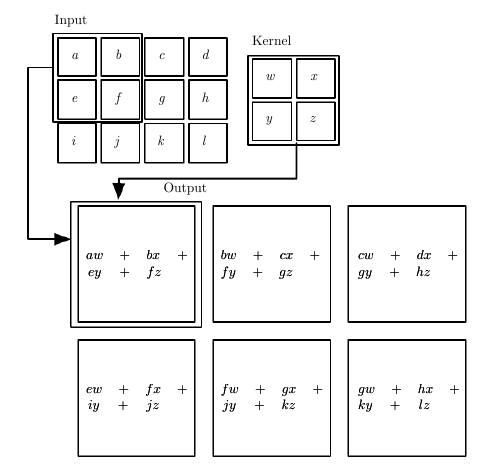
\includegraphics[width=.9\linewidth]{data/2d_cnn.png}
    \caption{Discrete convolution applied to an input-matrix}
    \label{2d_cnn}
\end{figure}

The input-matrix can represent an image, and the output is a matrix-like multiplication to a section of the input image which is the size of the kernel. This operation is repeated for all possible input values of the image.

In the typical CNN network terminology, the first argument is often refered to as the \textit{input}, the second argument is the \textit{kernel}, and the output by applying the convolution, is the \textit{feature map}.

As can be seen in Figure \ref{2d_cnn}, each output pixel results from applying the kernel to a small patch of the input image. These patches do overlap however and do can be bigger then in Figure \ref{2d_cnn}. Several kernels are trained and applied to the input image and thereby form the first convolutional layer.

The general Convolutional Network architecture consists of several convolutional layers stacked over each other, each of them followed by a pooling layer. Pooling layers perform, depending on their kind, a combination of a small output patch of the previous convolutional layer. Following figure \ref{max_pooling} shows a simple example of max-pooling, where only the maximum value of the convolutional layer's output is passed on as the output of the pooling patch.

\begin{figure}[H]
    \centering
    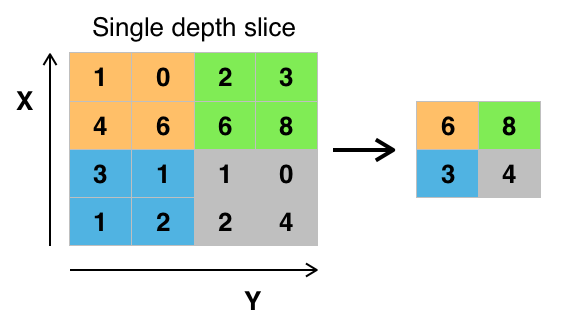
\includegraphics[width=.9\linewidth]{data/max_pooling.png}
    \caption{Max-pooling}
    \label{max_pooling}
\end{figure}

The outputs of the pooling layers form a filtered, lower-dimensional representation of the previous convolutional layer. By stacking pairs of convolutional- and pooling layers, the representations get more abstract with each layer and since each convolution and pooling operation reduces the dimensionality, the upper layers operate on a bigger scope of the input image.

The use of pooling-layers also makes the learned lower-level representations, i.e. features, invariant to small shifts in position. The reduction of dimensionality in depth with each layer is also called subsampling.

The following figure \ref{typical_architecture} shows the typical architecture of a Convolutional Neural Network.

\begin{figure}[H]
    \centering
    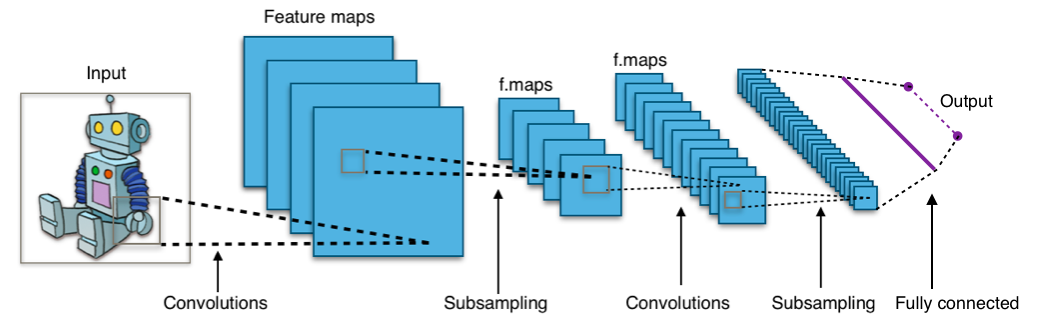
\includegraphics[width=\linewidth]{data/typical_cnn.png}
    \caption{Typical CNN architecture}
    \label{typical_architecture}
\end{figure}

After training several layers of convolution and subsampling (e.g. pooling) learned a fixed size and abstract representation of the input image. The last subsampling layer is then followed by several fully connected layers which act as a classifier to distinguish the image-classes present in the dataset. The complete architecture is then trained end-to-end (including the fully connected layers).

\subsection*{Intermediate CNN Results and Visualization}

Before performing any training on our data, we wanted to test the capabilities of the used framework \textit{Keras} on a well tested dataset. Therefore we trained a smaller model with 2D convolutional layers and max-pooling using the MNIST dataset (see Figure \ref{cnn_results_2}). In \ref{cnn_results_1} we show the results after the first convolutional layer. This model was trained using the Keras framework on top of Theano.

\begin{figure}[H]
    \centering
    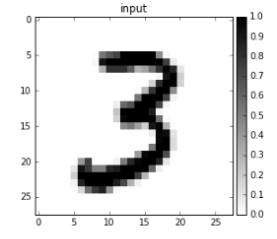
\includegraphics[width=0.8\linewidth]{data/cnn_results_2.png}
    \caption{Image taken from MNIST dataset. Every row and column represents one pixel size.}
    \label{cnn_results_2}
\end{figure}

The learned 32 kernels after the convolutional layer can be seen in the following image. 

\begin{figure}[H]
    \centering
    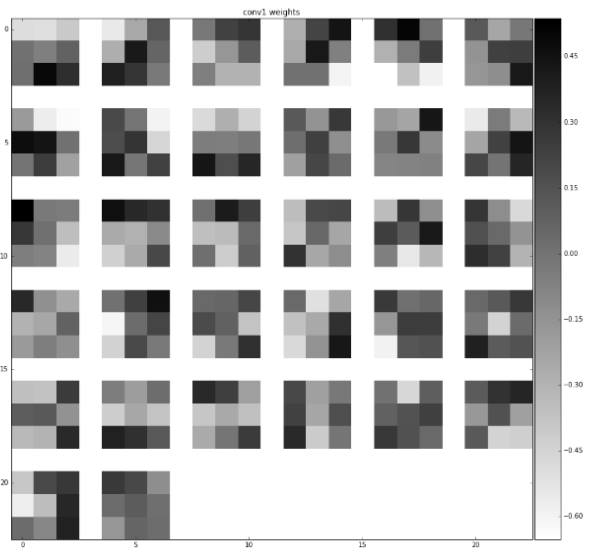
\includegraphics[width=0.8\linewidth]{data/cnn_results_3.png}
    \caption{All 32 kernels learned from the first convolutional layer.}
    \label{cnn_results_3}
\end{figure}

And the application of these filters or learned kernels to the image presented in \ref{cnn_results_2} is shown below. 

\begin{figure}[H]
    \centering
    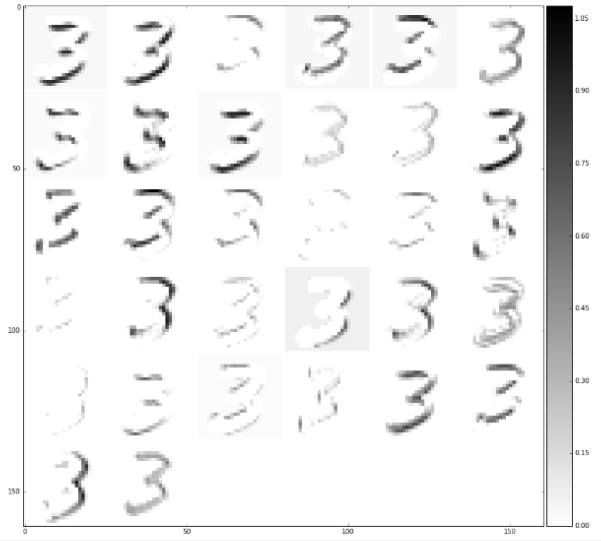
\includegraphics[width=0.8\linewidth]{data/cnn_results_4.png}
    \caption{All 32 Kernels applied to an example of the datase.}
    \label{cnn_results_4.png}
\end{figure}

We can observe that just after the first convolution layer, the model is able to distinguish the shape of the contours of the data. 

\subsection*{Sparse Coding}
----- Nitish's text here. -----

\section{Approach}

\subsection*{Datasets}
For training the final model we collected a datset consisting of a total of 424 Images of the following RoboCup@Home-Objects:
\begin{itemize}
    \item Pack of Coffee
    \item Paper coffee-cup
    \item Juice-box
    \item Big ketchup bottle
    \item Small ketchup bottle
    \item Mr Muscle cleaner
    \item Pepper
    \item Pringles can
    \item Water bottle
\end{itemize}

The pictures were taken with a low resolution camera (640x480 pixel) equivalently to the camera mounted on Jenny-COB, from a fixed angle and on a fixed background (white table).
The Images were then cropped and scaled to fit the network input size of 32x32 pixel.

Our datasets, as well as the implementation is available here: \begin{tiny}\url{https://github.com/oarriaga/machine_learning_algorithms/tree/master/algorithms/convolutional_neural_network}\end{tiny}

\subsection*{CNN-Architecture}
Our final model consists of 4 convolutional layers, each followed by a max-pooling layer. The first layer takes 32x32 pixels for each color channel (RGB) as inputs, resulting in 3*32*32 input units.
After the final max-pooling layer a two layered fully connected network is added as classifier. The final layer uses softmax-activation function, each previous layer uses rectified linear units.

\subsection{CNN-Training}
The model was trained using stochastic gradient descent with a learning-rate of $0.01$, weight-decay of $10^{-6}$ and momentum of 0.9 for 100 epochs.
Dropout is used in every layer to reduce overfitting.

The training dataset was splitted into a training-set (80\%) and a testing-set (20\%).

\subsection*{Sparse Coding}
----- Nitish's text here. -----

\section{Results}

\subsection*{CNN}
After 100 epochs of training, which took approximately ??, the model achieved an accuracy 98.55\%.

We took a cluttered picture by accident which has correctly been classified.

\begin{figure}[H]
    \centering
    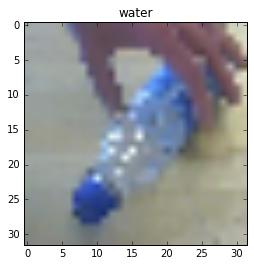
\includegraphics[width=0.5\linewidth]{data/cluttered_image}
    \caption{Cluttered image of the class "Water bottle" with hand of experimenter. The network was able to classify the image correctly.}
\end{figure}

When plotting the activations of convolutional layers, the abstraction and reduction in dimensionality that occurs can be made visible.

\begin{figure}[H]
    \centering
    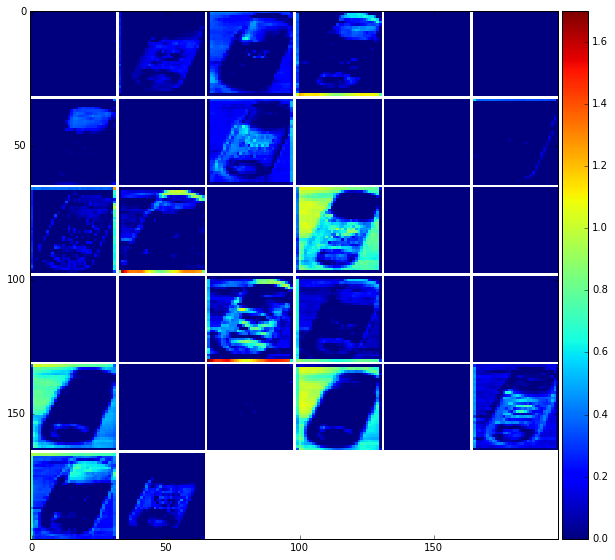
\includegraphics[width=0.5\linewidth]{data/final_cnn_firstlayer}
    \caption{Output after the first convolutional layer of our network, when presented with an input image.}
\end{figure}

\begin{figure}[H]
    \centering
    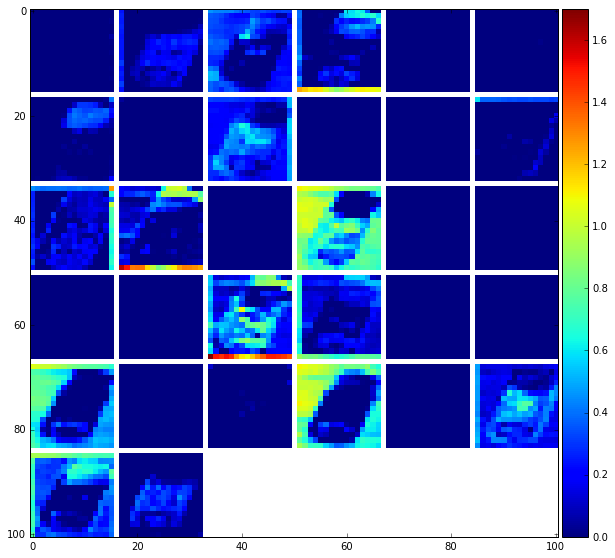
\includegraphics[width=0.5\linewidth]{data/final_cnn_secondlayer}
    \caption{Output after the second convolutional layer of our network, when presented with an input image.}
\end{figure}

\begin{figure}[H]
    \centering
    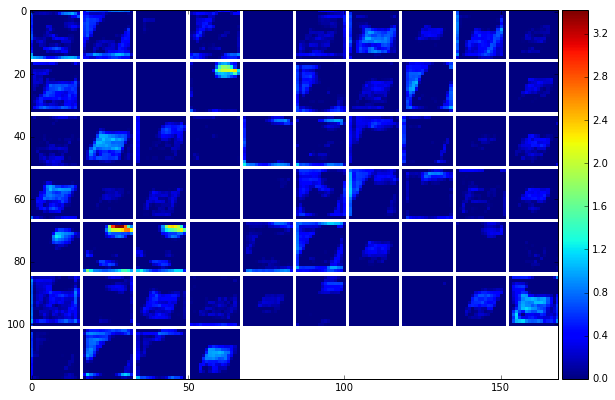
\includegraphics[width=0.5\linewidth]{data/final_cnn_thirdlayer}
    \caption{Output after the third convolutional layer of our network, when presented with an input image.}
\end{figure}

\begin{figure}[H]
    \centering
    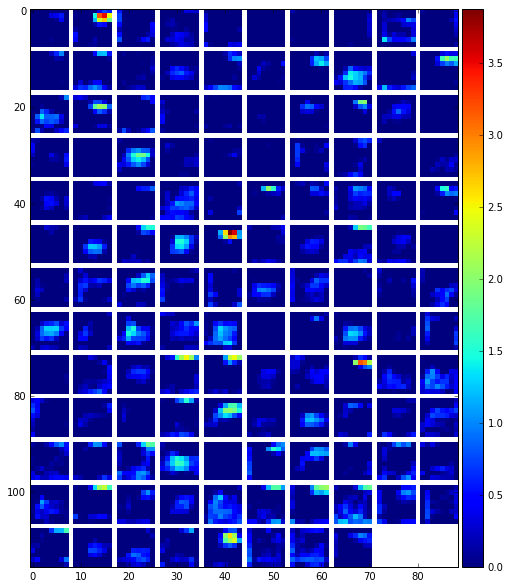
\includegraphics[width=0.5\linewidth]{data/final_cnn_fourthlayer}
    \caption{Output after the fourth convolutional layer of our network, when presented with an input image.}
\end{figure}

\subsection*{Sparse Coding}
----- Nitish's text here. -----

\section{Conclusion}

We implemented and trained a CNN on a dataset that we created from RoboCup@Home and RoboCup@Work objects. The results were very good, a real system could easily function with a classification accuracy of 98.55\%. 

In the future several issues should be addressed however. Since the dataset we created was relatively small, overfitting might be an issue. A second dataset could be created with the same objects but differnt conditions as lighting, background, occlusions and viewing angle. Artificial methods for enlarging the dataset, like applying small transformations could also be used.

\newpage

\section*{Sources}

\newpage

\onecolumn

\section*{Appendix B: Results}

\HorRule

\end{document}
